\begin{equation}
\langle \widetilde{\delta}_i ({\bf k}) \widetilde{\delta}_j ({\bf k'}) \rangle = (2 \pi) ^3 \delta_D \left( {\bf k} - {\bf k'} \right) P_{ij} \left({\bf k} \right)
\end{equation}

\begin{equation}
    \widetilde{\Delta} \left( k \right) = \frac{k^3}{2 \pi ^2} P \left( k \right)
\end{equation}

\begin{equation}
    \Delta \left( k \right) = \left( \nu I_{\nu} \right)^2 \widetilde{\Delta} \left( k \right)
\end{equation}s

\begin{figure}[ht]
	\centering
	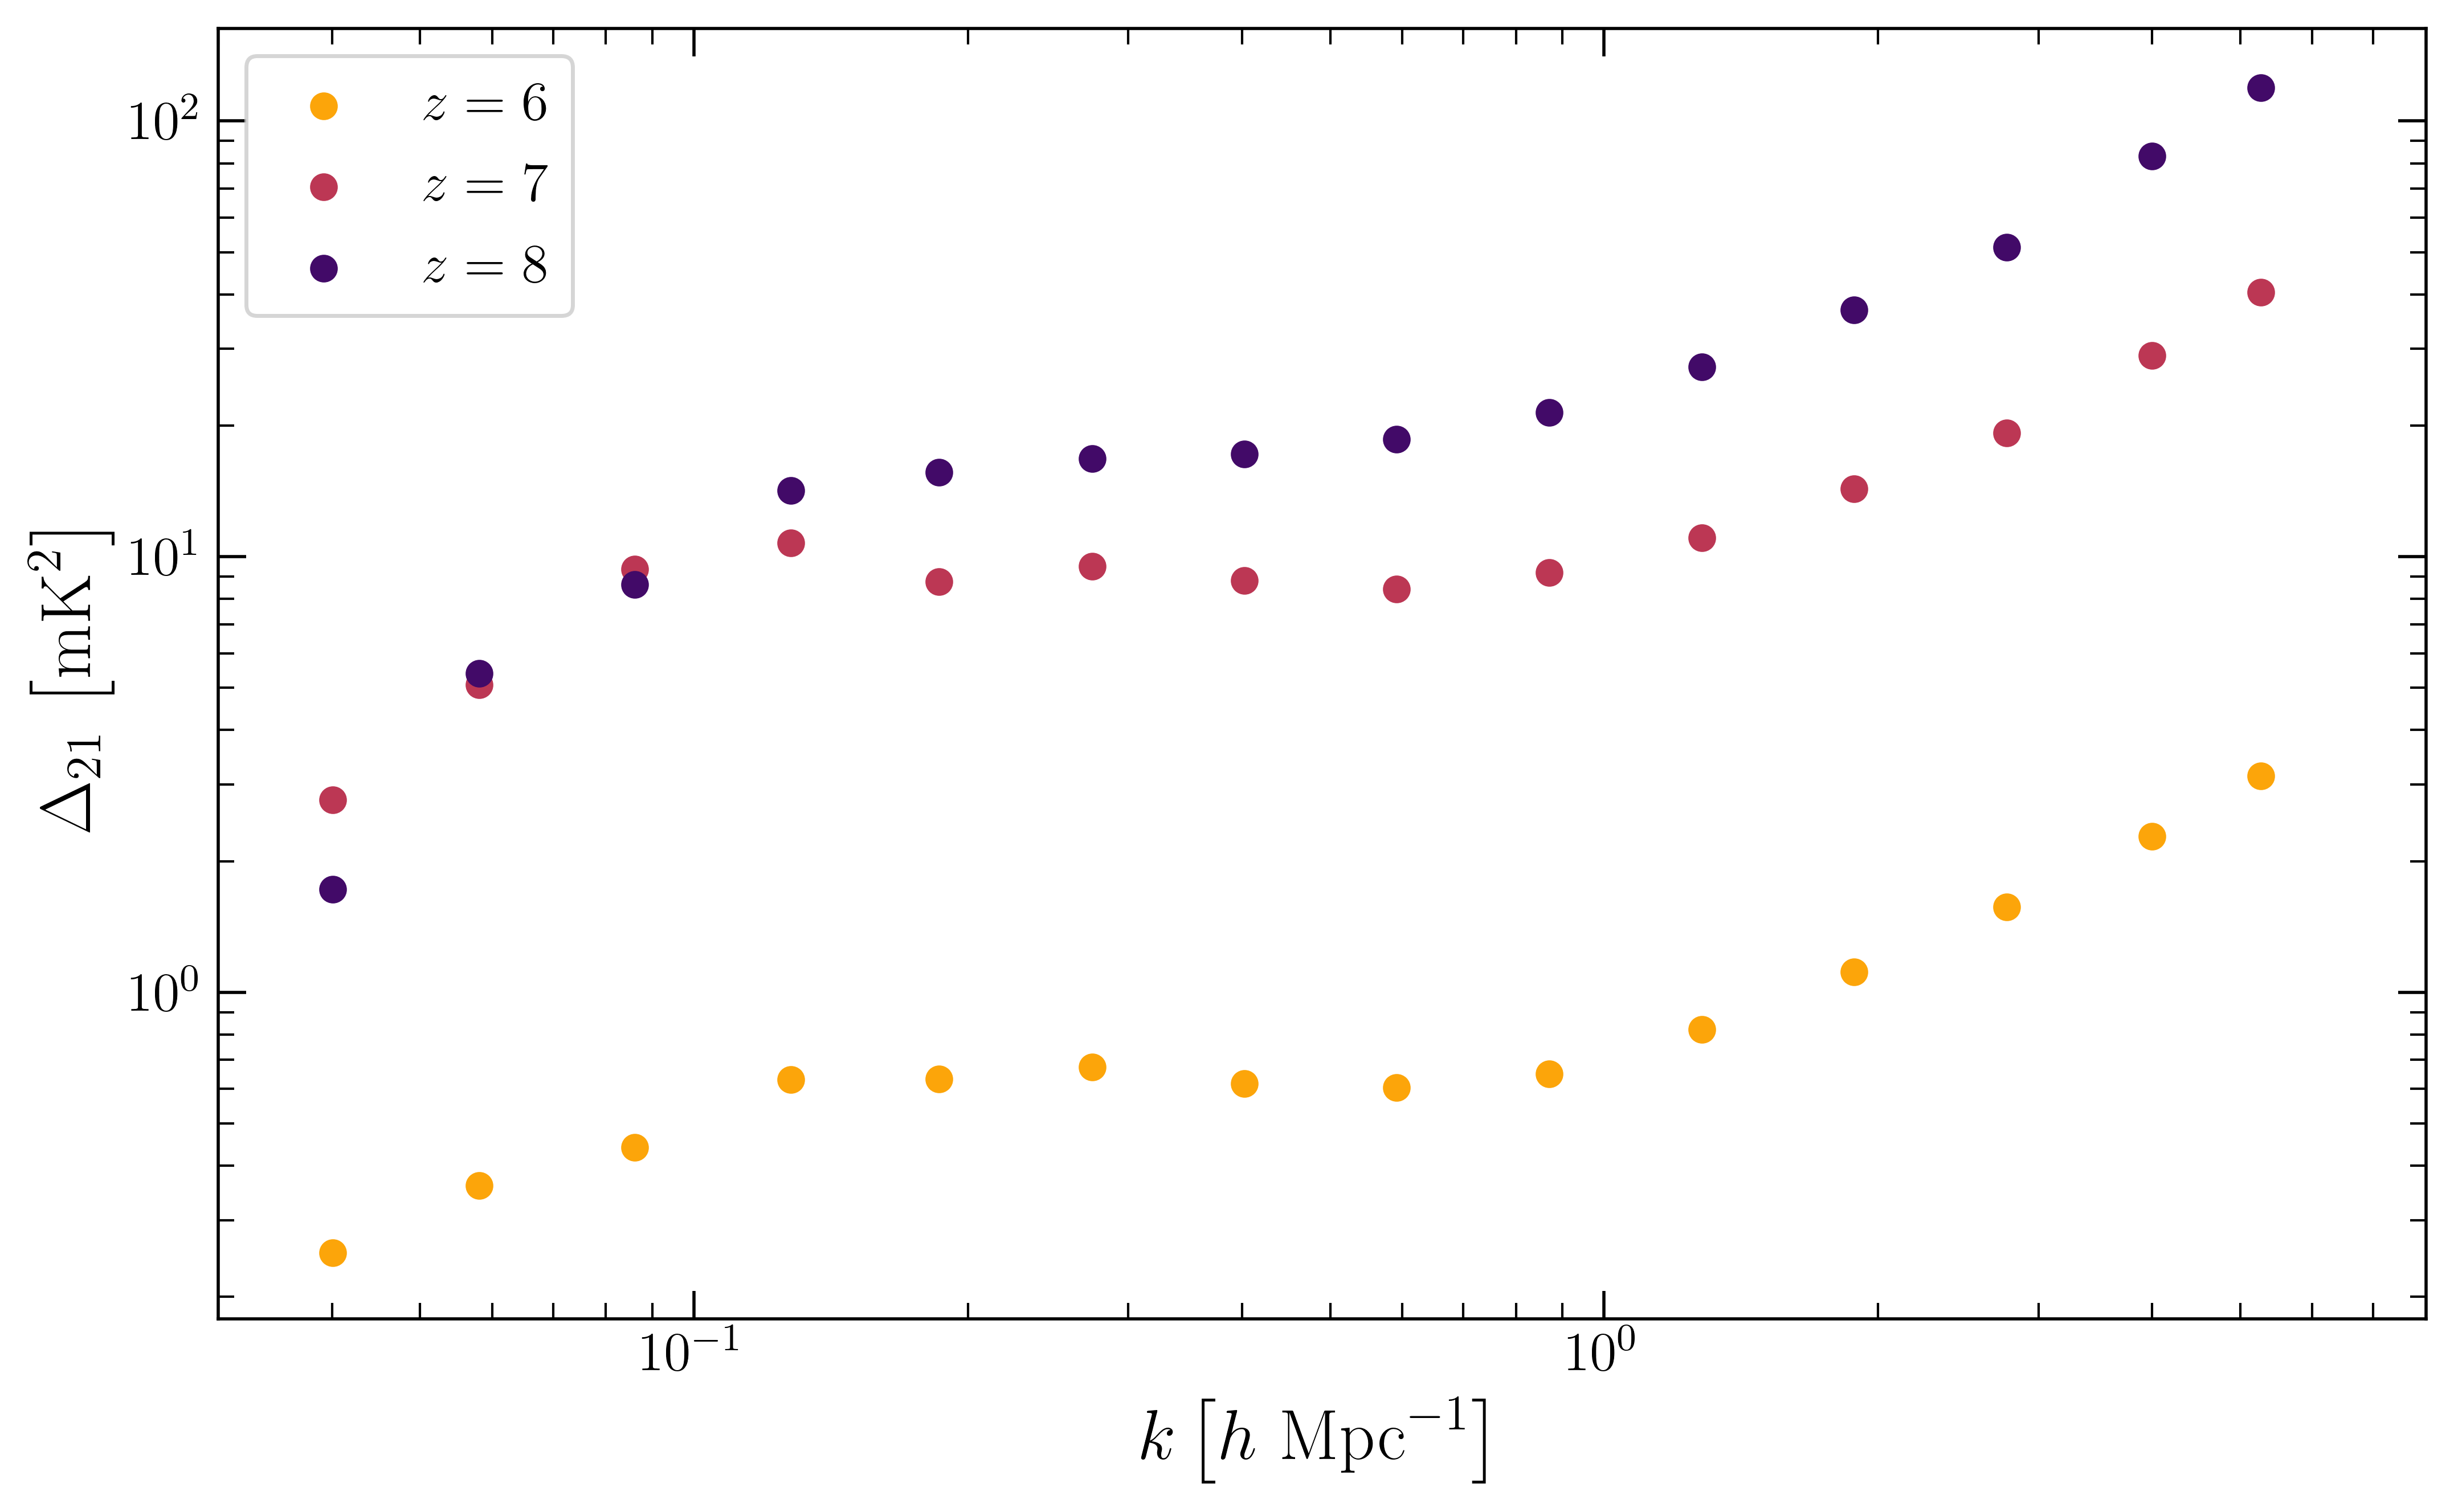
\includegraphics[width=0.9\textwidth]{21cm_power_spectrum.png}
	\caption[21cm Power Spectrum]{Cross-correlation coefficient}
	\label{fig:21cm_ps}
\end{figure}

\begin{figure}[ht]
	\centering
	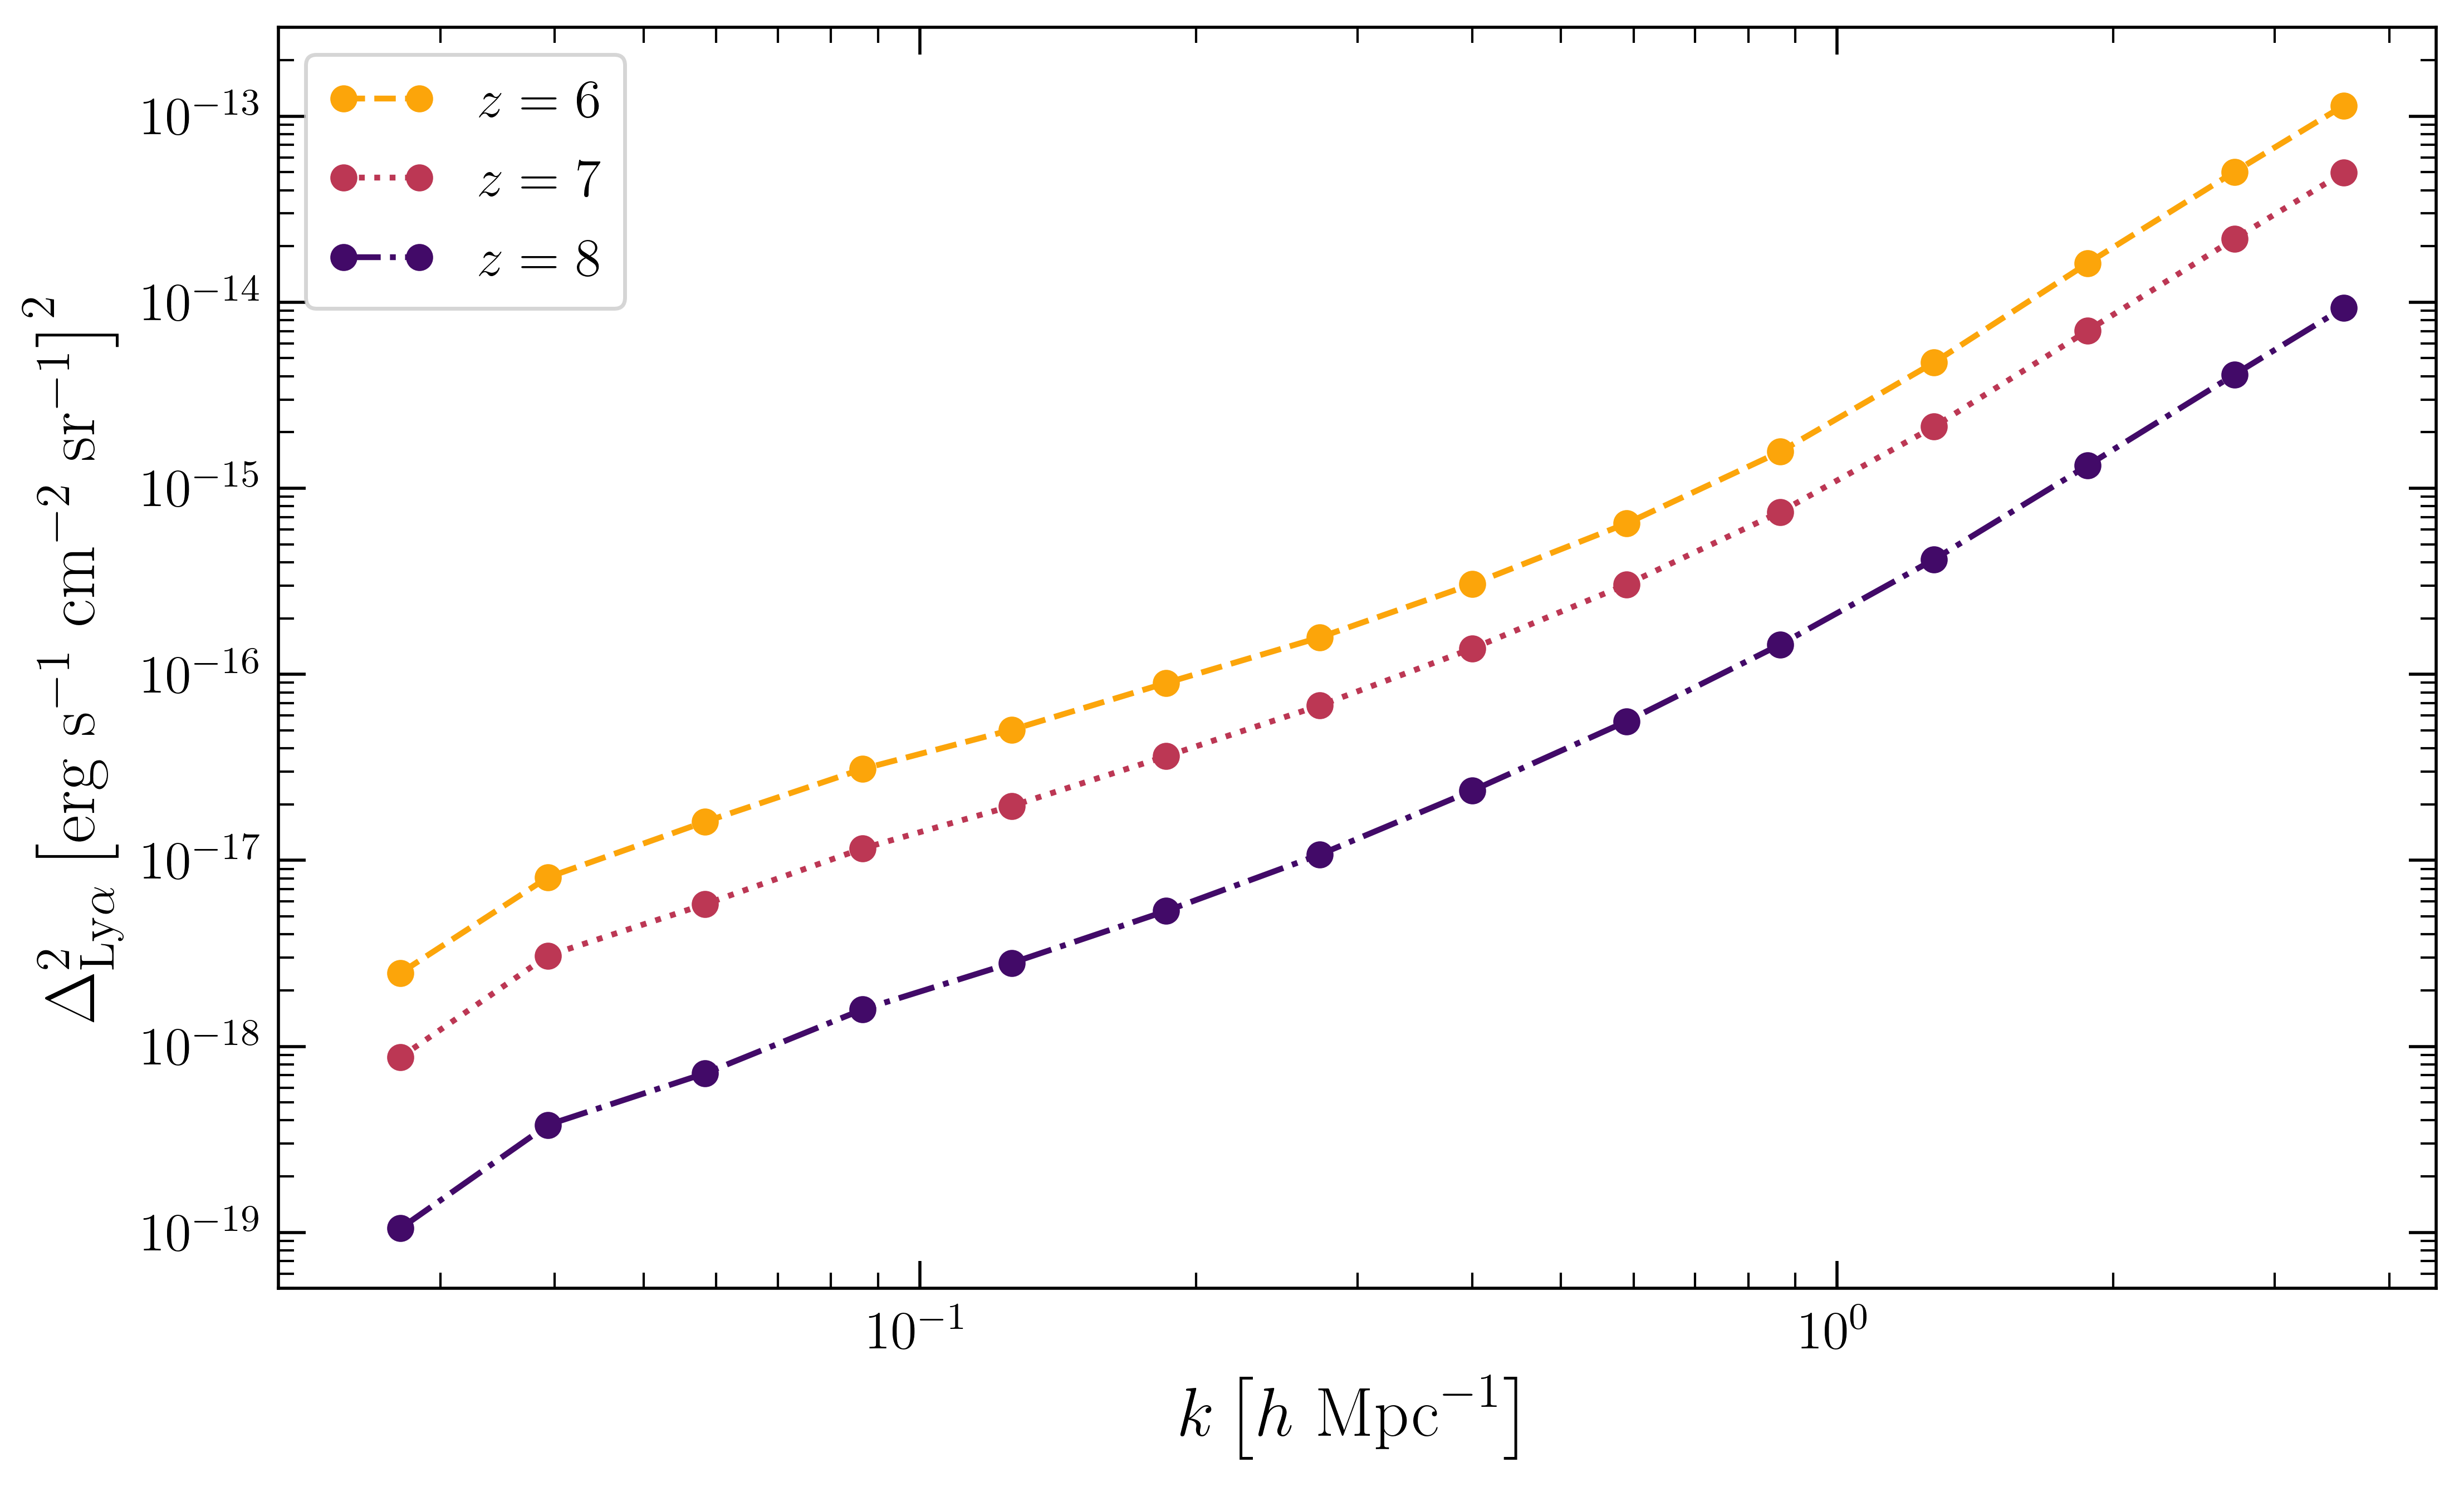
\includegraphics[width=0.9\textwidth]{lyman_alpha_pspec.png}
	\caption[Ly$\alpha$ Power Spectrum]{Cross-correlation coefficient}
	\label{fig:lya_ps}
\end{figure}

\begin{figure}[ht]
	\centering
	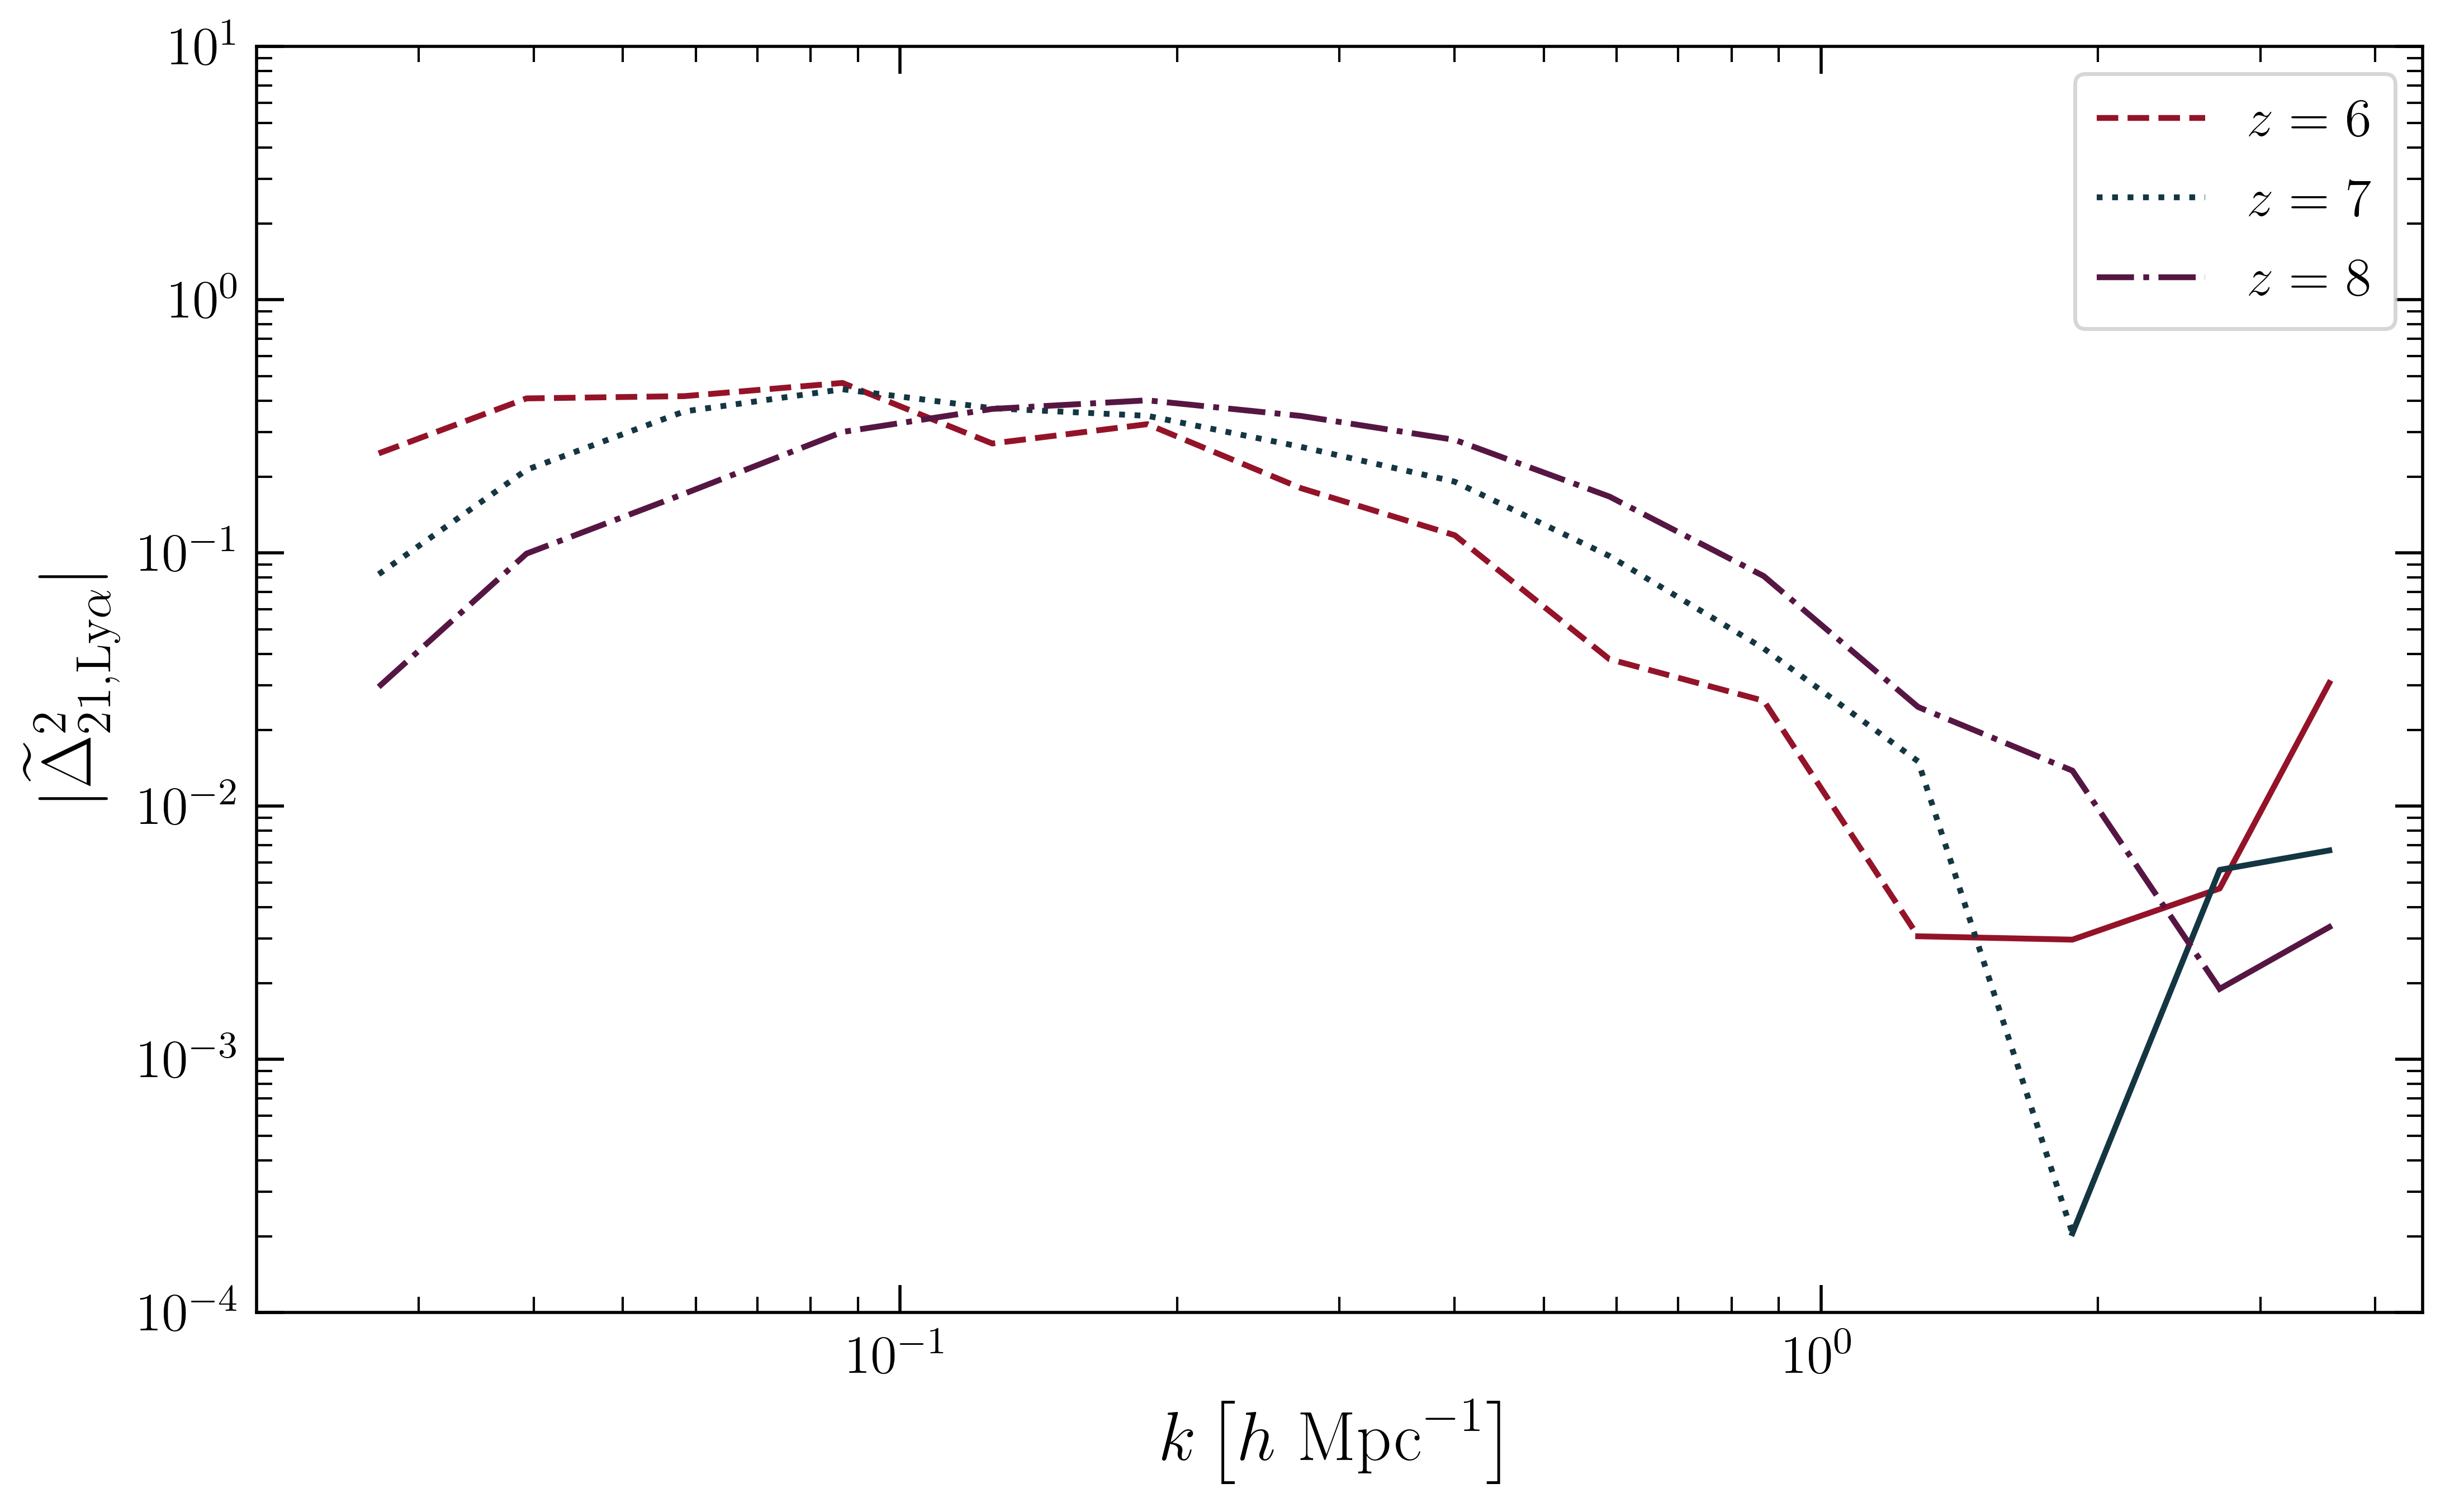
\includegraphics[width=0.9\textwidth]{cross_power_spec.png}
	\caption[Cross-Power Spectrum]{Cross-correlation coefficient}
	\label{fig:x_ps}
\end{figure}

\begin{figure}[ht]
	\centering
	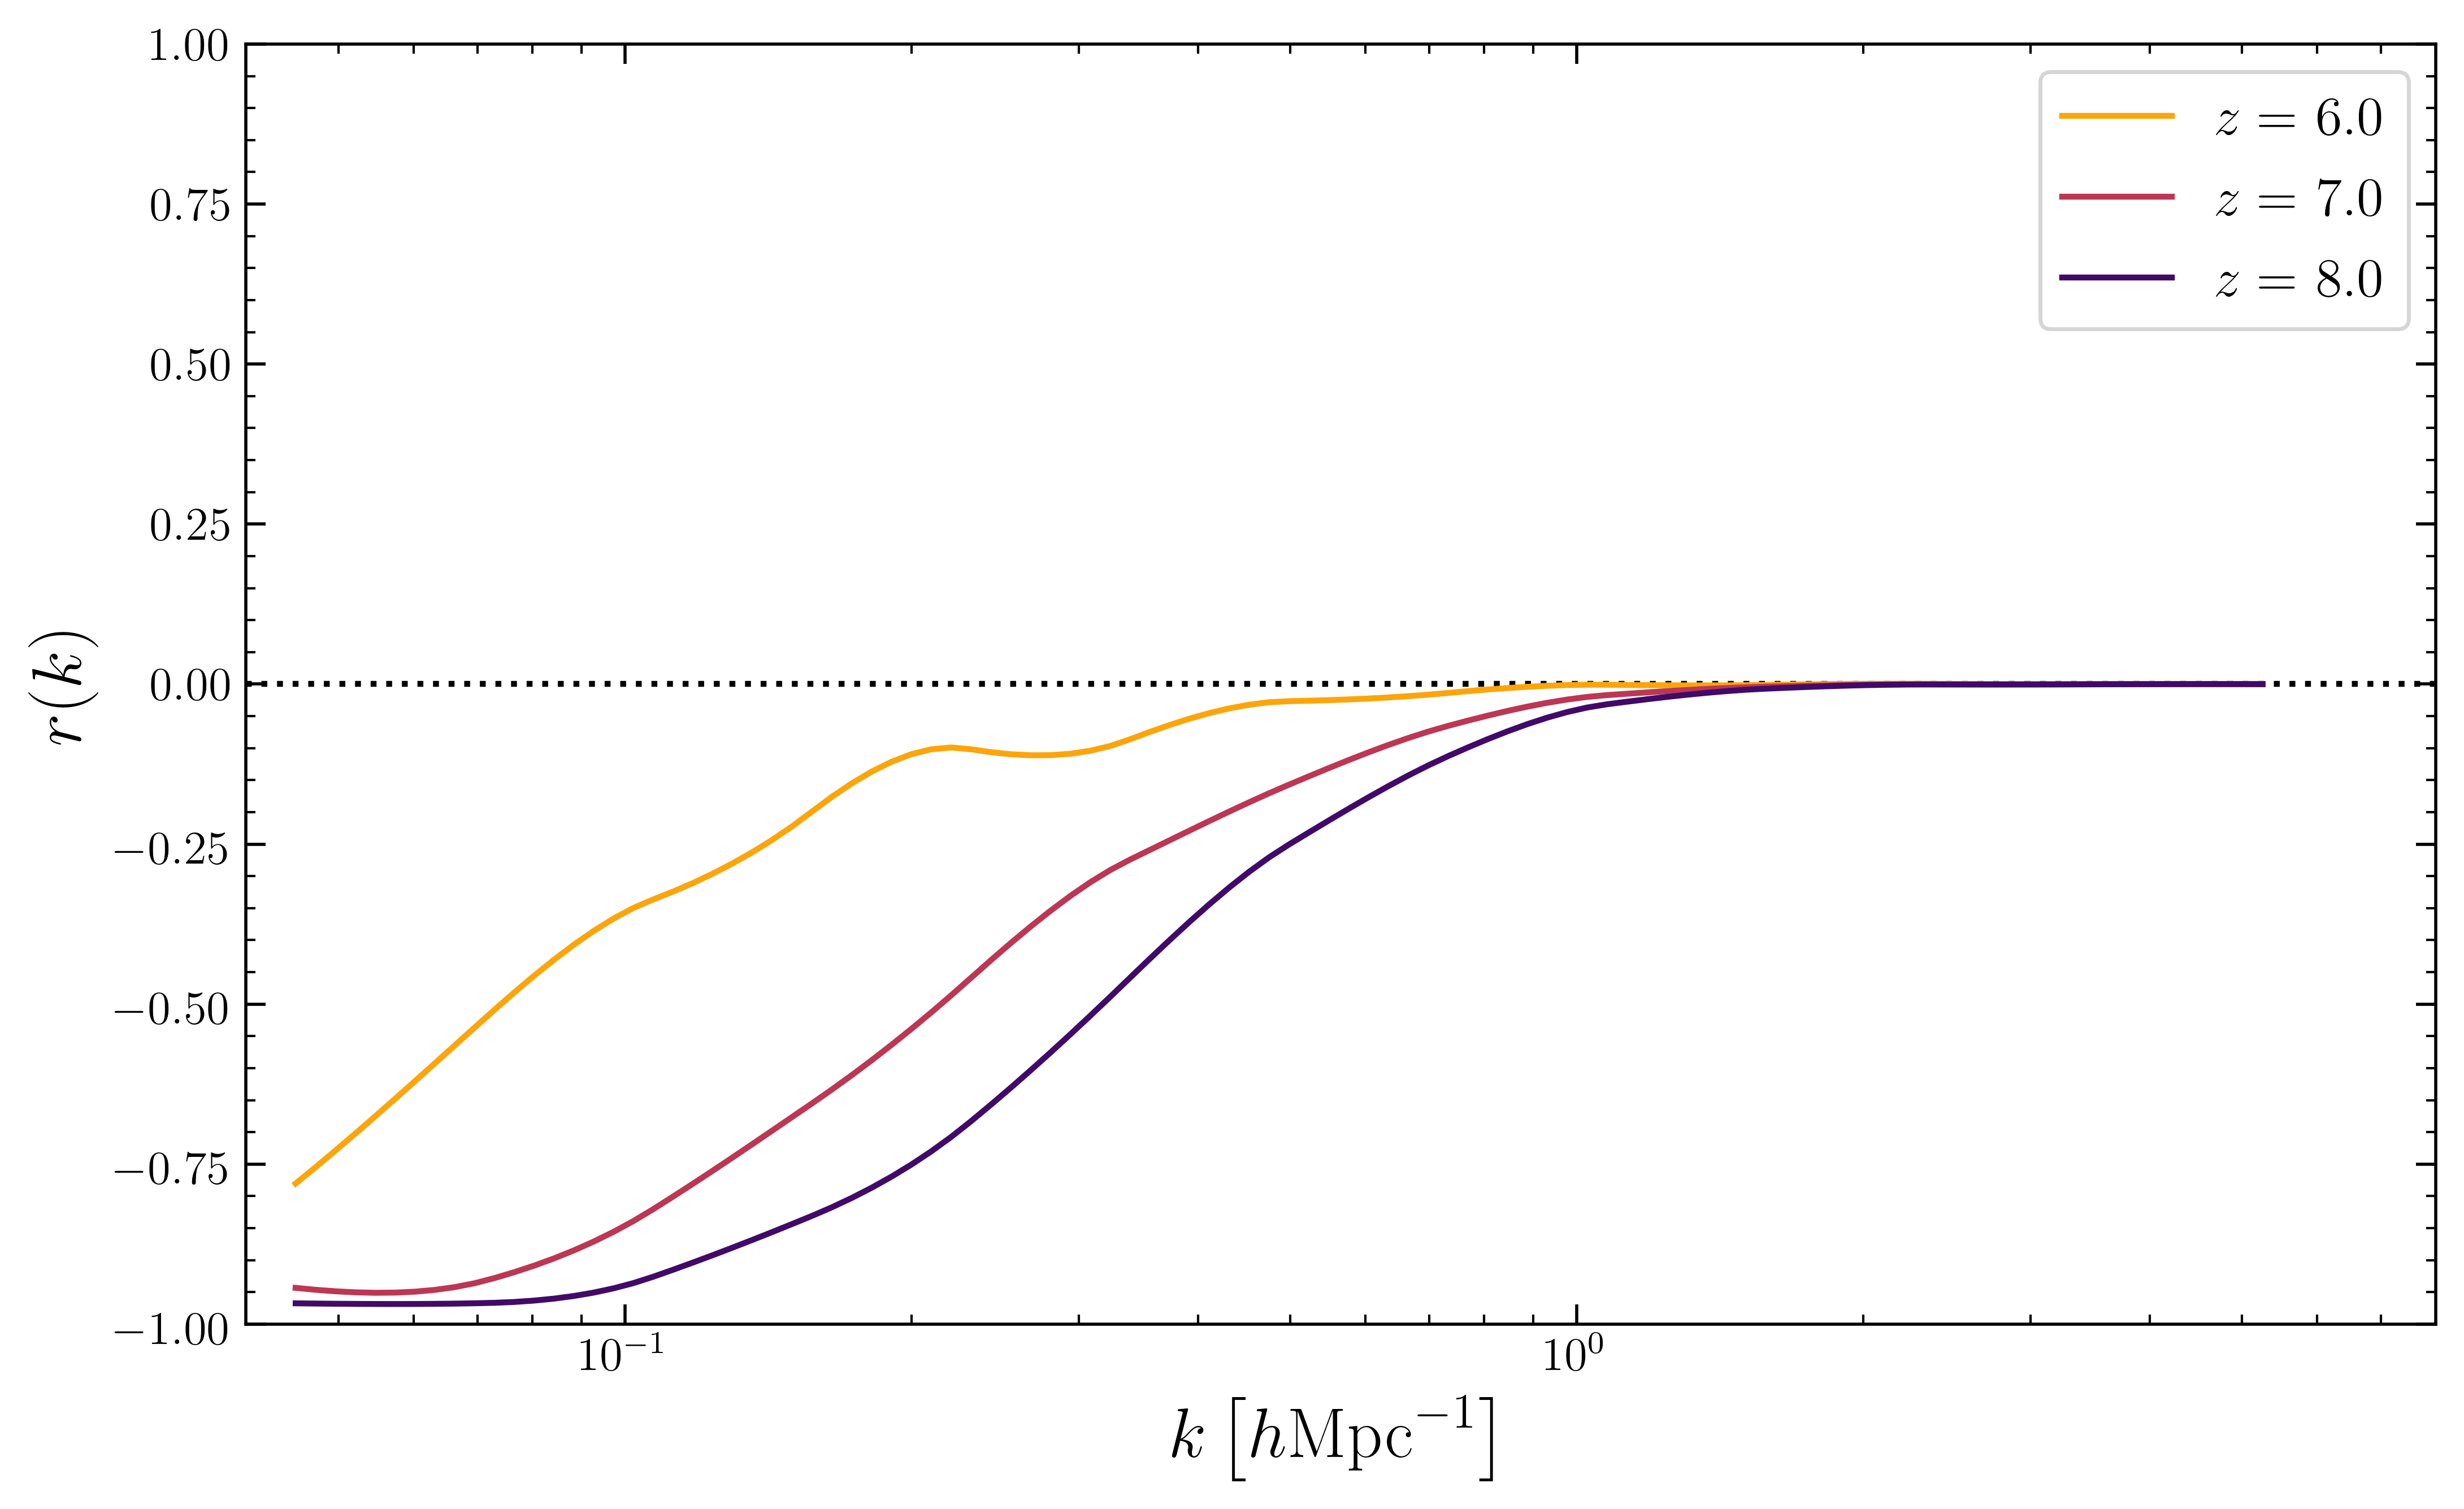
\includegraphics[width=0.9\textwidth]{ccc_plot.png}
	\caption[Cross-Correlation Coefficient]{Cross-correlation coefficient}
	\label{fig:ccc}
\end{figure}
